\section{Structure from Motion}
\label{structure}
Different than the previous section, in this section we are not using single point camera assumption.
Without this assumption, we cannot affirm that there is a projective transformation (homography) between two views.
In this section we will explain how we used Structure from Motion\cite{SfM} to create a set of 3D point clouds
representing the teddy bear shown in Figure~\ref{fig:bear}.

Using LO-RANSAC\cite{ransac} in combination with the eight-point algorithm\cite{eightpoint} and the Sampson distance,
we can estimate the fundamental matrix.
LO-RANSAC adds an improvement step to the results of every RANSAC-iteration.
If the amount of inliers of the iteration is above a certain ratio of the population this step is started.
In this improvement-step the inliers of the RANSAC-iteration are used as the population from which the actual model,
the fundamental matrix, is then calculated.

The eight-point algorithm derives the fundamental matrix with a sample of eight points.
We have used the normalized version that is better suited to derive the fundamental matrix.
This version transforms the points in such a way that the points have a mean distance of $\sqrt{2}$.

The fundamental matrix is a relationship between any two images of the same scene that constrains
where the projection of points from the scene can occur in both images.
These constraints are called the epipolar constraints.
An example of this can be seen in Figure~\ref{fig:epipolar}.
Here we see the lines that constrain the location of the points in the other image.
\begin{figure}[ht]
	\centering
	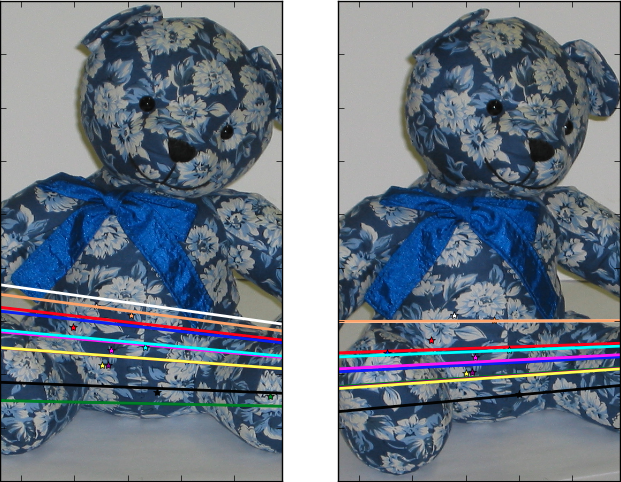
\includegraphics[width=.5\textwidth]{bear_epi}
	\caption{The epipolar constraints of two images of the teddy bear.}
	\label{fig:epipolar}
\end{figure}

The Sampson distance that is used to calculate the inliers is a approximation of the distance from a point to the epipolar lines.

We will use this to create a point view matrix, a matrix where the rows are images and columns are feature points in the images.
This matrix is of size $2m \times n$ where $m$ is the amount of cameras and $n$ the number of feature points that occur in 3 or more images. 
It is $2m \times n$ instead of $m \times n \times 2$ is so we can do Singuluar Value Decomposition.
With the results of this SVD we can create two matrices, the motion- and structure-matrices.
However as we can see in Figure~\ref{fig:pvm} not every point is seen in every image.
To deal with this we need to use a factorization method to still use Singular Value Decomposition to create a 3D point cloud that represents the teddy bear.
The factorization method that we have chosen to use is to extract dense subblocks from this point view matrix  and create multiple motion- and structure-matrices and stitch them together afterwards.

\begin{figure}[ht]
	\centering
	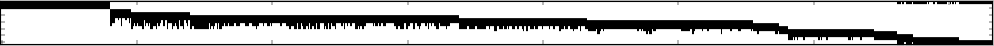
\includegraphics[width=\textwidth]{pvm}
	\caption{The point view matrix of the teddy bear. Black entries represent a value, whereas a white represents a point that is not seen in that image.}
	\label{fig:pvm}
\end{figure}

We have also eliminated the affine ambiguity by using a system of equations from the motion matrix and the Cholesky composition. This should improve the performance of our system.

In Figure~\ref{fig:points} the results of this part of the system are seen. The first image clearly shows the structure of the teddy bear. However other 3D points clouds are less clear about what they represent.

\begin{fig9ure}[ht]
	\subfloat[The first dense block of the PVM]{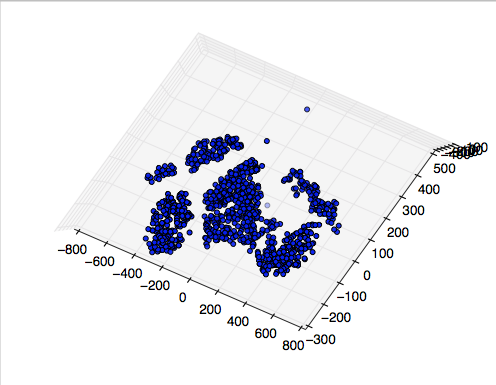
\includegraphics[width=.4\textwidth]{bear_points1}} \quad
	\subfloat[The second dense block of the PVM]{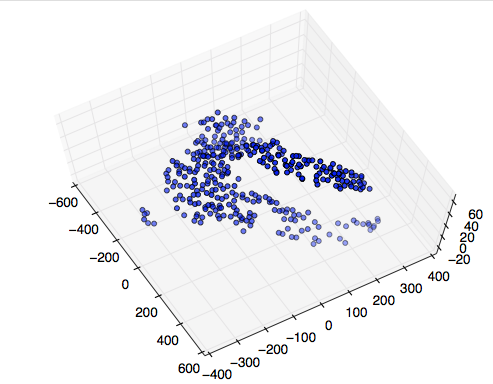
\includegraphics[width=.4\textwidth]{bear_points2}}
	\caption{The results of the Structure from Motion after the elimination of affine ambiguity. Left clearly shows the bear. Other results, like the right one are less clear.}
	\label{fig:points}
\end{figure}
